\documentclass[12pt, letterpaper, spanish]{article}
\usepackage{babel}
\usepackage[T1]{fontenc}
\usepackage{textcomp}
\usepackage[utf8]{inputenc} % Puede depender del sistema o editor
\usepackage{amsmath}
\usepackage{amsfonts}
\usepackage{amssymb}
\usepackage[left=2cm,right=2cm,top=2cm,bottom=2cm]{geometry}
\usepackage{mathrsfs}
\usepackage{pstricks-add}
\usepackage{pgfkeys}
\usepackage{setspace}
\usepackage{fancyhdr}
\usepackage{graphicx}
\usepackage{enumerate}

\usepackage{tikz}
\usetikzlibrary{fit,positioning}
\newcommand{\jump}{\vskip 0.01cm}
\begin{document}
\begin{titlepage}
	\centering
	{\scshape\LARGE Instituto Politécnico Nacional\\ Unidad Profesional Interdisiplinaria de Ingenierias campus Zacatecas\par}
	\vspace{1cm}
	{\scshape\Large Probabilidad Y Estadistica\par}
	\vspace{1.5cm}
	{\huge\bfseries Unidad 2 Tarea 1\par}
	\vspace{2cm}
	{\Large\itshape Gerardo Ayala Juárez\par}
	{\Large\itshape Olando Odiseo Belmonte Flores\par}
	{\Large\itshape Lucía Monserrat López Méndez\par}
	{\Large\itshape Oscar Iván Palacios Ulloa\par}
	\vfill
	Maestro:\par
	\textsc{
	Rosendo Vasquez Bañuelos}
	\vfill
% Bottom of the page
	{\large \today \par}
\end{titlepage}
\textbf{2.-} De tres ejemplos de variables aleatorias de Bernouli\vskip0.5cm

\textbf{4.-} Sea $X$ el número de dígitos no cero en un código postal seleccionado al azar. ¿Cuáles  son los posibles valores de $X$? Dé tres posibles resultados y sus valores $X$ asociados.\\
4 (cuatro ceros)\\
3 (tres ceros)\\
2 (dos ceros)\\
1 (un cero)\\
0 (cero ceros)\\
98087 ($X=1$), 01000 ($X=4$), 98000($x=3$) \vskip0.5cm

\textbf{6.-} A partir de una hora fija, cada carro que entra a una intersección es observado para ver si da vuelta a la izquierda (L), la derecha (R) o si sigue de frente (A). El experimento termina en cuanto se observa que un carro da vuelta a la izquierda. Sea $X$ el número de carrosobservados. ¿Cuáles son los posibles valores de $X$? De cinco resultados y sus valores $X$ asociados.\\
$X = x,\ x=1,2,3,4,...$\\
RAAL ($X=4$), L ($x=1$), ARL ($X=3$), RARRARL ($X=7$), RL ($X=2$) \vskip0.5cm
\textbf{22.-}Una empresa de ventas en línea dispone de seis líneas telefónicas. Sea X el número de líneas en uso en un tiempo especificado. Suponga que la función masa de probabilidad de X es la que se da en la tabla adjunta. Calcule y trace la gráfica de la función de distribución acumulativa F(x). Luego utilícela para calcular las probabilidades de los eventos dados en los incisos a)–d) de dicho problema. \vskip 0.01 cm
\begin{tabular}{l|c c c c c c c}
    x&0&1&2&3&4&5&6\\
    \hline
    p(x)&0.10&0.15&0.20&0.25&0.20&0.06&0.04\\
\end{tabular}\\
\textbf{24.-}Una compañía de seguros ofrece a sus asegurados varias opciones diferentes de pago de primas. Para un asegurado seleccionado al azar, sea $X$el número de meses entre pagos sucesivos. La función de distribución acumulativa es la siguiente:\vskip 0.01 cm
\begin{center}
F(x)=$\left\{\begin{array}{l c}
    0 & x<1\\
    0.30 & 1 \leq x < 3\\
    0.40 & 3 \leq x < 4\\
    0.45 & 4 \leq x < 6\\
    0.60 & 6 \leq x < 13\\
    1    & 12 \leq x\\
\end{array}\right.$
\end{center} \jump
\textbf{Respuestas.$\_$}\jump
\begin{itemize}
    \item[b):] Calcule lo siguiente.
    \jump $P(3\leq x \leq 6) =$ F(6)-F(1)= 0.60 - 0.30 = .30
    \jump $P(x \leq 4) =$ f(0)+f(1)+f(3)+f(4) = F(4)=0.15
    \item[a):] ¿Cuál es la función de masa de probabilidad de X?
    \jump \begin{center} $\begin{array}{c c c c c c c}
        f(12)&=&F(12)-F(6)&=&1.0 - 0.60&=&.040\\
        f(6)&=&F(6)-F(4)&=&0.60 - 0.45&=&0.15\\
        f(4)&=&F(4)-F(3)&=&0.45 - 0.40&=&0.05\\
        f(3)&=&F(3)-F(1)&=&0.40 - 0.30&=&0.10\\
        f(1)&=&F(1)-F(0)&=&0.30 - 0.0&=&0.30\\
        f(0)&=&F(0)&=&0 &=&0.00\\
    \end{array}$  \jump
    \begin{tabular}{l|c c c c c c}
        x&1&3&4&6&12\\
        \hline
        p(x)&0.30&0.10&0.05&0.15&0.40\\
    \end{tabular}
\end{center}
\end{itemize}
\textbf{26.-} Alvie Singer vive en 0 en el diagrama adjunto y sus cuatro amigos viven en A, B, C y D. Un día Alvie decide visitarlos, así que lanza al aire una moneda imparcial dos veces para decidir a cuál de los cuatro visitar. Una vez que está en la casa de uno de sus amigos, o regresará a su casa o bien proseguirá a una de las dos casas adyacentes (tales como 0, A o C, cuando está en B) con cada una de las tres posibilidades cuya probabilidad es $\displaystyle\frac{1}{3}$. De este modo, Alvie continúa visitando a sus amigos hasta que regresa a casa.
\jump
\begin{center}
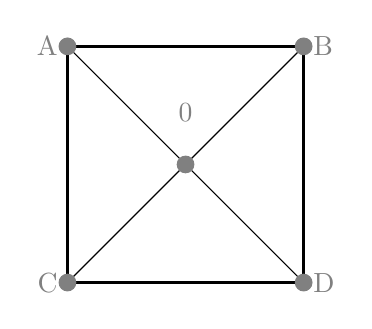
\begin{tikzpicture}
 
    \draw[ very thick] (0,0) rectangle (3,3);
    \draw (0,0) -- (3,3) (0,3) -- (3,0);
    \filldraw[gray]
  (0,0)       circle (3pt) node [align=left,   left  ] {C}
  (3,3)       circle (3pt) node [align=left,   right ] {B}
  (0,3)       circle (3pt) node [align=left,   left  ] {A}
  (3,0)       circle (3pt) node [align=left,   right ] {D}
  (1.5 , 1.5) circle (3pt) node [align=left,   above ] {0\\};
    \end{tikzpicture}
\end{center}    
\begin{itemize}
    \item[a)]Sea X = el número de veces que Alvie visita a un amigo. Obtenga la función masa de probabilidad de X.\jump
    \textbf{Respuestas.$\_$}\jump
    x=1,2,3,4\jump 
    $\left\{\begin{array}{cc}
        \frac{1}{4}&\frac{1}{3}\\
        A&0\\
        B&0\\
        C&0\\
        D&0\\
    \end{array}\right\}$ = 1 \hspace{0.1cm}
    $\left\{\begin{array}{ c c c}
        \frac{1}{4}&\frac{1}{3}&\frac{1}{2}\\
        A&B&0\\
        B&C&0\\
        C&D&0\\
        D&A&0\\
        A&D&0\\
        B&A&0\\
        C&B&0\\
        D&A&0\\
    \end{array}\right\}$ = 2 \hspace{0.1cm}
    $\left\{\begin{array}{c c c c }
        \frac{1}{4}&\frac{1}{3}&\frac{1}{2}&\frac{1}{2}\\
        A&B&C&0\\
        B&C&D&0\\
        C&D&A&0\\
        D&A&B&0\\
        A&D&C&0\\
        B&A&D&0\\
        C&B&A&0\\
        D&A&B&0\\
    \end{array}\right\}$= 3 \hspace{0.1cm}
    $\left\{\begin{array}{c c c c c }
        \frac{1}{4}&\frac{1}{3}&\frac{1}{2}&\frac{1}{2}&1\\
        A&B&C&D&0\\
        B&C&D&A&0\\
        C&D&A&B&0\\
        D&A&B&C&0\\
        A&D&C&B&0\\
        B&A&D&C&0\\
        C&B&A&D&0\\
        D&C&A&B&0\\
    \end{array}\right\}$= 4 \jump
    $\begin{array}{l|c c c c}
        x&1&2&3&4\\
        \hline
        p(x)&\frac{1}{3}&\frac{1}{3}&\frac{1}{6}&\frac{1}{6}
    \end{array}$
    \item[b)]Sea Y = el número de segmentos de línea recta que Alvie recorre (incluidos los que conducen a o que parten de 0). ¿Cuál es la función masa de probabilidad de Y?
    \textbf{Respuestas.$\_$}\jump
    y=2,3,4,5\jump 
    $\left\{\begin{array}{cc}
        \frac{1}{4}&\frac{1}{3}\\
        A&0\\
        B&0\\
        C&0\\
        D&0\\
    \end{array}\right\}$ = 2 \hspace{0.1cm}
    $\left\{\begin{array}{ c c c}
        \frac{1}{4}&\frac{1}{3}&\frac{1}{2}\\
        A&B&0\\
        B&C&0\\
        C&D&0\\
        D&A&0\\
        A&D&0\\
        B&A&0\\
        C&B&0\\
        D&A&0\\
    \end{array}\right\}$ = 3 \hspace{0.1cm}
    $\left\{\begin{array}{c c c c }
        \frac{1}{4}&\frac{1}{3}&\frac{1}{2}&\frac{1}{2}\\
        A&B&C&0\\
        B&C&D&0\\
        C&D&A&0\\
        D&A&B&0\\
        A&D&C&0\\
        B&A&D&0\\
        C&B&A&0\\
        D&A&B&0\\
    \end{array}\right\}$= 4 \hspace{0.1cm}
    $\left\{\begin{array}{c c c c c }
        \frac{1}{4}&\frac{1}{3}&\frac{1}{2}&\frac{1}{2}&1\\
        A&B&C&D&0\\
        B&C&D&A&0\\
        C&D&A&B&0\\
        D&A&B&C&0\\
        A&D&C&B&0\\
        B&A&D&C&0\\
        C&B&A&D&0\\
        D&C&A&B&0\\
    \end{array}\right\}$= 5 \jump
    
    \begin{center}
        F(y)=
        $\left\{\begin{array}{cc}
            0            & y <2 \\
            \frac{1}{3} &2\leq y < 3\\
            \frac{2}{3} &3\leq y < 4\\
            \frac{5}{6} &4\leq y < 5\\
            1           & y\leq 5
        \end{array}\right.$
    \end{center}
    \item[c)]Suponga que sus amigas viven en A y C y sus amigos en B y D. Si Z = el número de visitas a amigas, ¿cuál es la función masa de probabilidad de Z?    
    \textbf{Respuesta$\_$}\jump
    z=0,1,2 \jump
    $\left\{\begin{array}{ccc}
        \frac{1}{12}&B&0\\
        \frac{1}{12}&D&0\\
    \end{array}\right\}$ = 0 \hspace{0.1cm}
    $\left\{\begin{array}{ c c c c c}
        \frac{1}{12}&A&0& &\\
        \frac{1}{12}&C&0& &\\
        \frac{1}{24}&A&B&0&\\
        \frac{1}{24}&A&D&0&\\
        \frac{1}{24}&B&A&0&\\
        \frac{1}{24}&B&C&0&\\
        \frac{1}{24}&C&B&0&\\
        \frac{1}{24}&C&D&0&\\
        \frac{1}{24}&D&A&0&\\
        \frac{1}{24}&D&C&0&\\
        \frac{1}{48}&B&A&D&0\\
        \frac{1}{48}&B&C&D&0\\
        \frac{1}{48}&D&A&B&0\\
        \frac{1}{48}&D&C&B&0\\
    \end{array}\right\}$ = 1 \hspace{0.1cm}
    $\left\{\begin{array}{c c c c c c}
        \frac{1}{48}&A&B&C&0&\\
        \frac{1}{48}&A&D&C&0&\\
        \frac{1}{48}&C&B&A&0&\\
        \frac{1}{48}&C&D&A&0&\\
        \frac{1}{48}&A&B&C&D&0\\
        \frac{1}{48}&B&C&D&A&0\\
        \frac{1}{48}&C&D&A&B&0\\
        \frac{1}{48}&D&A&B&C&0\\
        \frac{1}{48}&A&D&C&B&0\\
        \frac{1}{48}&B&A&D&C&0\\
        \frac{1}{48}&C&B&A&D&0\\
        \frac{1}{48}&D&C&A&B&0\\
    \end{array}\right\}$= 2 \jump
    \begin{center}
    $\begin{array}{l|c c c}
        z&0&1&2\\
        \hline
        p(z)&\frac{2}{12}&\frac{7}{12}&\frac{3}{12}\\
    \end{array}$
\end{center}
\end{itemize}
\end{document}
